\documentclass{notes}
\graphicspath{{Visualizations/}}

\fancyhead[l]{Jonathan Cheng, Holden Kowitt, Finnegan Wright}
\fancyhead[c]{}
\fancyhead[r]{December 13, 2024}
\fancyfoot[c]{Page \thepage\ of \pageref{LastPage}}
\bibliographystyle{IEEEtran}

\begin{document}

\subsection*{Capstone Project Report}

\subsection*{Introduction}

The aim of this project was to effectively model a fission nuclear reactor using python. The general structure is as follows. Beginning with a set number of neutrons, a Monte Carlo simulation was run to determine the number of fission, scattering, absorption, and escaped neutron events. Determining which events happen utilizes the cross-sections of the different materials in the reactor. A cross-section is a measure of area and can be used to determine the mean free path or the probability of an interaction happening, dependent on the particular elements involved and the energy of a given neutron. Using the cross-sections, cumulative density functions can be found which are used in the simulation. 

With the number of different events, several interesting physical properties of the reactor can be calculated. Primarily, whether the reactor produces as many neutrons as it consumes; i.e. is the reactor critical. Other results include (but are not limited to) the number of antineutrinos the reactor produces, how much power the reactor produces, or how the criticality changes as the concentrations of materials are changed in the reactor.

\subsection*{Implementation}

\subsubsection*{Our Process}

Reaching our final desing took several iterations, as multiple hurdles had to be overcome before we reached a workable model. This process saw us first simulating a single neutron, turning this model into a crude Monte Carlo. As we worked towards a more polished model, we split our code into several interacting modules. These modules would first spawn a set number of neutrons into the simulation, process their interactions based on their cross-sections (probabilities), and produce counts of each event which occurred. These three modules, in order, may be referred to as the `neutrons' modeule (initialize\verb|_|neutrons), the `density' module (density\verb|_|functions), and the `escape' module (check\verb|_|escape). Finally a fourth `master' file would be used to bring each of these pieces together by initializing the reactor size, number of neutrons, the particular elements involved, and then running each of the other modules. This final file was labeled the `reactor' module (reactor\verb|_|function) in the final iteration.

The second significant update put in much of the work to create cohesion between the modules. It updated the escape module so that event counters could be reset within the module itself, and created a consistently functional reactor module. A visualization module (reactor\verb|_|visualizations) module was also added, allowing for several graphical displays of input-output interactions. This ultimately helped us verify how realistic our reactor was, allowing us to visualize several known aspects of nuclear reactors as well as indicating places where there was room to improve our simulation. Many of the graphics from this visualization module will be shown in the results section below. Finally, upon noticing in our visualizations that our base reactor wasn't nearing criticality, we added a variation of our escape module that allowed for partial reflection (rather than escape), providing more realism as well as demonstrating criticality.

\subsubsection*{Code Walkthrough}

\textbf{Neutrons Module}

The neutron module creates a `neutrons' function which takes as inputs the number of neutrons (count), the reactor radius, and the energy of each neutron (array-like). Firstly, a (3, 3, count) array is initialized with random values between 0 and 1. Each neutron was represented by a slice along axis 2 and needed to represent an (x, y, z) position, direction, and an energy. The first row's random (0, 1) was used to give each neutron a randomized spherical coordinate which was then converted to cartesian. The second row indicated the direction (x, y, z) the particle would travel, and was converted to unit length. The neutron energies (an input to the original function) would be placed in the position (2,0), with the final 2 positions in the array unused.

\textbf{Mixtures Module}

By unpacking and processing a csv file, we receive the cross-sectional information on uranium-238 \cite{Kim, Andersen}, uranium-235, boron-10 \cite{Bogart}, and heavy water \cite{CrossSections}. When initiating a `mixtures' function, we inputted percentage values of the total reactor volume to be taken up by each material. These weighted densities allow us to show the probability of each event (fission, absorption, scattering) for both high- and low-energy neutrons. These new weighted cross-sections can then be used as inputs to our probability density function.

\textbf{Density Module}

The density function was somewhat simpler. Firstly, the probability density function takes the number of particles and total cross section as inputs, outputting a function of `x'. The cumulative distribution function integrates over the pdf. By taking the inverse of the cdf and mapping onto it a random value (0, 1), we find the distance each particle will travel before experiencing an interaction. \cite{OpenMC}

\textbf{Escape Module (No Reflection)}

The escape module creates a 1d array which, using the inverse cdf function, determines the distance each neutron will travel before an interaction. By moving the particle's position in the specified direction, it will receive a final position. If this position is outside the reactor, the neutron will have successfully escaped; else it will perform a different event based on the probabilities taken from the mixtures module. In the case that the neutron scatters, its energy may be decreased and it will be run through the simulation recursively.

\textbf{Reflective Shell}

A variation of the escape module allowed neutrons to reflect off a wall rather than simply escaping. This was done probabilistically depending on a certain defined reflectivity. By making this change, our reactor was much more real-to-life and could reach a critical level.

\textbf{Reactor File}

The reactor file is the main file which gets run, calling each of the others as necessary. By having all the alterable variables in one place, it is very easy to run and see how changes in input affect each of the simulated results.

\subsection*{Results}

Following the completion of our reactor simulation, we coded several visualization functions focused specifically on generating graphs. These visualized how our simulation reacted to shifting input variables and can be broadly categorized into two groups: material and criticality graphics.

\subsubsection*{Material Graphics}

Material graphics focused on varying the percentages of our material inputs and seeing how our counters reacted.

Looking first at uranium percentages, we are able to demonstrate the impact of enrichment on fission by making a graphic which ran our simulation from 1\% enrichment (99\% U-238, 1\% U-235) to 100\% enrichment. This graph showed us that the largest gains stopped at 20\% but the number of fissions still continued to increase slowly. This matches perfectly with real world use-cases, where the vertical lines on the graph separate natural uranium, reactor-grade uranium, and weapons-grade uranium.

Our second material graphic sought to observe the impact of a moderator on the amount of scattering within the reactor. By varying the percentage of moderator (heavy water) from 1-66\% (higher percentages would result in a non-reactive fuel), with 20\% enriched uranium, the increase was close to linear.

For the last materials graphic, we could see the impact of control rod insertion on the reactivity of a reactor; how power plants `poison' their reactors to prevent meltdown. By varying the percentage of boron from 1-75\% against fission counts, the graphic showed a rapid decrease in fissions with increasing quantities of boron.

\begin{figure}[H]
    \centering
    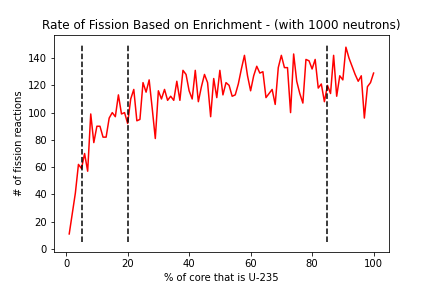
\includegraphics[width = 0.3\textwidth]{enrichment.png}
    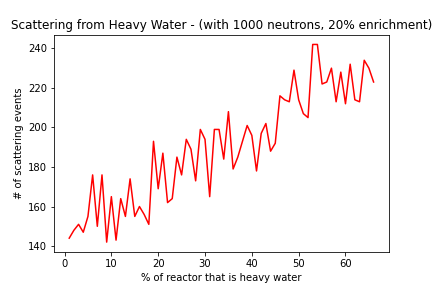
\includegraphics[width = 0.3\textwidth]{heavy_water.png}
    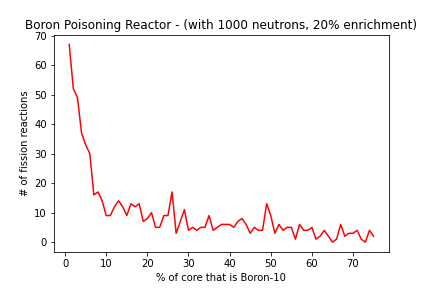
\includegraphics[width = 0.3\textwidth]{boron.png}
    \caption{Enrichment, Moderator, Boron Poisoning (left to right)}
\end{figure}

\subsubsection*{Criticality Graphics}

Our first criticality graphic used the model without reflectivity and sought to test if criticality was possible with a sufficiently large reactor core. By starting with 1000 neutrons, we looked for the value of reactor radius where the number of neutrons produced from fission exceeded this initial amount, given that the average number of neutrons produced from each fission was 2.5.

Following this same process with a 50\% reflective shell showed that criticality could occur at a lower reactor radius if reflection was accounted for.

\begin{figure}[H]
    \centering
    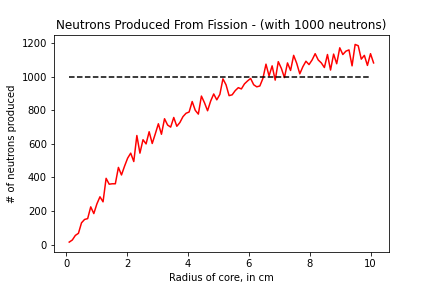
\includegraphics[width = 0.3\textwidth]{criticality_radius_nr.png}
    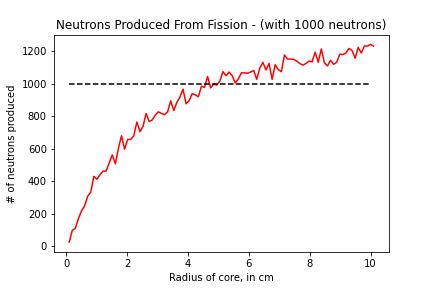
\includegraphics[width = 0.3\textwidth]{criticality_radius_r.png}
    \caption{Criticality without (left) and with (right) reflection}
\end{figure}

The last criticality graphics illustrated the ways in which enrichment and reflectivity impact reactivity. The first graphic varied the reflectivity (rather than the radius) and graphed against the number of neutrons produced.

Similarly, a second graph varied the number of neutrons produced by the level of uranium enrichment.

\begin{figure}[H]
    \centering
    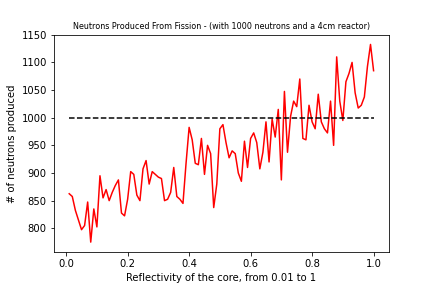
\includegraphics[width = 0.3\textwidth]{criticality_reflectivity_r.png}
    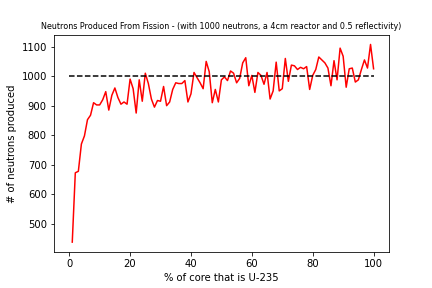
\includegraphics[width = 0.3\textwidth]{criticality_enrichment_r.png}
    \caption{Criticality vs. reflectivity (left); Criticality vs enrichment (right)}
\end{figure}

\subsection*{Discussion}

Looking at our graphical results, we see much to indicate the quality of simulation, particularly in its accuracy reflecting the mechanisms and characteristics of real-world reactors. 

One particularly notable example is in the enrichment of uranium. Unenriched uranium, in the 1-5\% range, is clearly much worse for fusion, improving quickly through the 5-20\% reactor-grade enrichment. At higher levels of enrichment, the rate of return diminishes but is still non-negligible. This matches the idea that reactor-grade uranium attempts to be efficient while cost effective. However for weapons, which intend maximum yield, it is sensible to use highly enriched uranium.

Our control rod graph shows, unsurprisingly, that more rods leads to a decrease in fissions. Excitingly, our reactor showed that 10\% boron pushes fission rates to near-zero: very close to the 5-10\% of volume used in real reactors to kill a reaction.

Our criticality graphs show that size, enrichment, and reflection all increase the potential for a critical reactor. This is necessary for energy production, but also demonstrates how dangerous reactors can be without mechanisms for moderation, leading to the possibiliity of going supercritical.

For small volumes, we saw that an open system was `safe,' however once reflections were added, the reactor fuel could become critical. Quickly producing high amounts of radiation from fissions is the same process which made the notorious `demon core' so deadly.

\subsection*{Concluding Remarks}

Overall, this simulation was very effective in what we set out to achieve. We saw the expected trends that should be seen, despite various assumptions made during the process of programming the simulation.

Throughout our process, the use of matricies and function mapping rather than loops led to significant speed improvements. As a group our work on the physics, code, presentation, and write-up were well balanced, as we learned to work individually as well as combining our efforts. One area we could improve is working in parallel on different tasks by separating modules early. What we did instead was work on the ideas sequentially and separated only for reasons of organization, leading to a slower group workflow.

If we wanted a more accurate model, there are a few directions which could significantly expand the project's scope. One such task would be using neutrons that are born with some distribution acros the `fast' energy regime and having unique energy loss from different scattering events. This would involve new cross-sections as well as certain numerical integration problems due to the cumulative distribution function. Another improvement might be to include time-dependence which, along with computational power, would require an inclusion of components such as fuel burnup, temperature, and fission products. Finally, we might model real reactor and control rod geometries rather than assuming homogeneity.

\nocite{*}
\bibliography{Capstone_Citations}

\end{document}